% setup the document and include packages
\documentclass{article}[12pt]
\usepackage{graphicx}
\usepackage{amsmath}
\usepackage{amssymb}
\usepackage{cancel}
\usepackage{ntheorem}
\usepackage{algorithm2e}
\usepackage{float}
\usepackage{caption}
\usepackage{fancyvrb}
\usepackage[dvipsnames]{xcolor}
\usepackage[section]{placeins}
\usepackage[toc,page]{appendix}
\usepackage{hyperref}
\usepackage{subfig}

%set stuff for syntax highlighting
%\usepackage{fontspec}
%\usepackage{minted}
%\setsansfont{Calibri}
%\setmonofont{Consolas}
\usepackage{hyperref}
\hypersetup{
    colorlinks=true,
    linkcolor=blue,
    filecolor=magenta,      
    urlcolor=cyan,
}
\urlstyle{same}

\makeatletter
\def\BState{\State\hskip-\ALG@thistlm}
\makeatother

% define Continue for algorithms
\SetKw{Continue}{continue}

% redefine QED symbol
\renewcommand{\qedsymbol}{\rule{0.7em}{0.7em}}

% define lemma and result theorem-styled sections
\newtheorem{lemma}{Lemma}[section]
\newtheorem{result}{Result}[section]

% setup paths for images
\graphicspath{ {../scripts/plots/} }

% Don't print the semicolon in algorithms
\DontPrintSemicolon

% define the title that will be used in the report
\title{CS 440 MP3 \\ Section Q4 \\ 4 Credits}
\author{
Christian Howard \\ howard28@illinois.edu
}
\date{} % don't set a date because we don't need this shit


% start the document
\begin{document}
   
   % create the title page 
   \maketitle
   \begin{abstract}
   Within this MP, software was developed to create and evaluate a Maximum a Posteriori classifier. This generic software was applied to a set of problems such as classifying handwritten digits, classifying face vs. non-face images, classifying Hebrew 'Yes' vs. 'No', and classifying spoken digits. The algorithms developed performed reliably, classifiers reaching at least 80\% accuracy with some reaching more than 95\% classification accuracy. Within the handwritten digits classifier and face classifier problems, some work was done into investigating the value and time complexity of using various block feature representations based on the original image data. It was found that there is a sweet spot in terms of feature block sizes that will have the best accuracy. Additionally, theoretical complexity trends were validated against experimental time measurements recorded during the training and testing phases of the handwritten digit classification process, helping to better contrast the pros and cons of the different feature representations.
   \end{abstract}
   \newpage
   
   % create table of contents on separate page
   \tableofcontents
   \newpage
   
   % start section covering work on Part 1.1
   \section{Naive Bayes Formulation} \label{sec:one}
   
   %%
   %% Subsection for Naive Bayes classifier formulation
   %%
   \subsection{Bayes Rule Classifier Formulation}
   Before diving into each of the problems for this MP, a discussion of the general mathematical formulation is an important first step and will allow for easily formulating the problems later.
   
   Let us assume our goal is to develop a classifier that can take some input $x \in \mathcal{X} = \mathcal{V}^d$, where $\mathcal{V} = \lbrace v_1, v_2, \cdots, v_m\rbrace$ are the values a component of $x$ can take, and produce some class $\omega \in \Omega = \lbrace \omega_1, \cdots, \omega_p \rbrace$ that is most likely representative when the input $x = v$, where $v$ is some value in $\mathcal{X}$. We can choose the classifier to be the following:
   
   \begin{align}
   \omega^* &= \arg \max_{\omega \in \Omega} P(\omega | x = v) \label{eq:c1}
   \end{align}
   
   Now using Bayes Rules and a Conditional Independence assumption, we can use the following relationship to compute the classifier:
   
   \begin{align*}
   P(\omega | x) &= \frac{P(\omega) P(x = v | \omega) }{\sum_{\hat{\omega} \in \Omega} P(x = v| \hat{\omega} ) P( \hat{\omega} )} \\
   &= \frac{ P(\omega) \prod_{l=1}^d P(x_l = v_l | \omega) }{\sum_{\hat{\omega} \in \Omega} P(x = v| \hat{\omega} ) P( \hat{\omega} )}
   \end{align*}
   
   Since the denominator is just a normalization constant shared between each $P(\omega | x = v)$, we can ignore computing it and just use the numerator to help choose the class. This means the classifier rule actually ends up being:
   
    \begin{align}
   \omega^* &= \arg \max_{\omega \in \Omega} P(\omega) \prod_{l=1}^d P(x_l = v_l | \omega) \label{eq:c2}
   \end{align}
   
   To make things more reasonable to compute in practice due to finite precision, without changing the classifier result, we can $\log\left(\cdot\right)$ the terms in the classifier:
   
   \begin{align}
   \omega^* &= \arg \max_{\omega \in \Omega} \log P(\omega) +  \sum_{l=1}^d \log P(x_l = v_l| \omega) \label{eq:c3}
   \end{align}
   
   
   %%
   %% Subsection for discrete value feature training
   %%
   \subsection{Learning with Discrete valued Features} \label{ssec:ldv}
   Based on \ref{eq:c3}, it is obvious that $P( \omega)$ and $P(x_l = \hat{v} | \omega)$ need to be computed $\forall \omega, x_l, \hat{v}$. As discussed in the MP problem statement, usage of Laplace Smoothing will be utilized to smooth the categorical data and make the algorithms we use more robust. 
   
   Let us assume we have some training dataset of inputs and label outputs $D_T$, defined as $D_T \subset D = \lbrace (x, \omega) | x \in \mathcal{X}, \omega \in \Omega \rbrace$. Let us define $G_{\omega}: \Omega \times D \rightarrow \mathcal{P}(\mathcal{X})$ as a map that, given some class and dataset, produces a subset of the input data that corresponds to the class $\omega$. Using this, we can define the computation for each of the desired probabilities as the following:
   
   \begin{align}
   P(\hat{\omega}) &= \frac{|G_{\omega}(\hat{\omega}, D_T)|}{|D_T|} \label{eq:po}\\
   P(x_l = \hat{v} | \hat{\omega}) &= \frac{ \alpha + \sum_{ \hat{x} \in G_{\omega}(\hat{\omega}, D_T) } \mu(\hat{x} \cdot \hat{e}_l, \hat{v}) }{ \alpha |\mathcal{V}| +  |G_{\omega}(\hat{\omega}, D_T)|} \label{eq:pxo}
   \end{align}
   
   where $\alpha$ is the Laplace Smoothing constant and $\mu: \mathcal{V}^2 \rightarrow \mathbb{R}$ is defined as the following:
   
   \begin{align}
   \mu(v_1, v_2) &= \begin{cases}
   1 & v_1 = v_2 \\
   0 & v_1 \neq v_2
   \end{cases}
   \end{align}
   
   These quantities are computed for each $\hat{\omega} \in \Omega, \hat{v} \in \mathcal{V}$, and each component of $x$. With these equations, the training can be done quite simply. To get a feel for the space and time complexity, the naive time complexity for computing (\ref{eq:po}) is $O(pN)$, where $N = |D_T|$, with a memory complexity of $O(p)$. As for (\ref{eq:pxo}), this quantity can be computed in $O(dmpN)$ with a space complexity of $O(dmp)$. Additionally, if we want to then evaluate this model after training, we can find the evaluation time complexity to be $O(pd)$ for each input point.
   
   
   \subsection{Implementation Discussion}
   Given the theoretical representation discussed above, the implementation was designed to allow for generic abstraction so I could tackle new problems by just modifying some of the defining quantities, like $d$, $V$, $\Omega$. The code basically implemented a Discriminant class that would take some dataset for a class, a Laplace Smoothing constant, and the total amount of data and produce a trained object that could compute class posteriors and likelihoods. Then, a separate function would take a list of these Discriminant objects and would perform the MAP computation for some set of input data.
   
   To keep things separate, I implemented methods to read in the data from disk in a manner that allowed me to pass in some functor that could transform the baseline input data into data with new features. I used this to easily go from the baseline pixel features to Disjoint and Overlapping block features, for example, with lots of code reuse. This allowed me to separate data reading and feature extraction from the classifier model in a very modular way.
   
   
   
   
   
   
   %%
   %% Section about Digit Classification
   %%
   \section{Problem 1 | Digit Classification}
   
   %%
   %% Subsection about Part 1.1 using pixel values as features
   %%
   \subsection{Single Pixels as Features} \label{ssec:spf}
   \subsubsection{Problem Formulation}
   Within this problem, we are handed a dataset of square images, each with $n = 28$ rows and columns, read into storage with binary values at each pixel. For ease of use, each image is vectorized into a column vector such that $V = \lbrace 0, 1 \rbrace $ and $d = n^2$, given the definitions in Section \ref{sec:one}. Note that we also define $\Omega = \lbrace 0, 1, \cdots, 9\rbrace$, where each value is a label for the corresponding hand-written digit. Using this formulation, it is trivial to use the generic algorithms based on the formulation in Section \ref{sec:one} to train and test the classifier.
   
   \subsection{Results}
   After a training run-time of around $0.155$ seconds and testing run-time of around $18.08$ seconds, the classifier was able to achieve an overall classification accuracy of $77.1$\%. The individual classification accuracy for each digit can be seen in Table \ref{tab:digacc}. This optimal classification was found with a Laplace Smoothing constant of $\alpha = 0.1$. I found that increasing the Laplace Smoothing constant actually hurt the training performance, which I found interesting. 
   
   \begin{table}[ht]
   	\centering
   	\begin{tabular}{l | c }
   		\hline
   		Digit & Classification Accuracy  \\
   		\hline \hline 
   		0 & 84.4\% \\
   		1 & 96.2\% \\
   		2 & 77.6\% \\
   		3 & 79.0\% \\
   		4 & 76.6\% \\
   		5 & 67.3\% \\
   		6 & 75.8\% \\
   		7 & 72.6\% \\
   		8 & 60.1\% \\
   		9 & 80.0\% \\
   		\hline
   	\end{tabular}
   	\caption{Accuracy for individual digit classifiers} \label{tab:digacc}
   \end{table}
   
   If we look at the Confusion Matrix in Figure \ref{fig:cm11}, we can see that most of the misclassifications were when it misclassified 4 as 9, misclassified 5 as 3, misclassified 7 as 9, and misclassified 8 as 3. When thinking about the shapes of these digits, these misclassifications seem reasonable. For each of these misclassification pairs, we see their associated log likelihood and log odds ratio plots in Figures \ref{fig:mdp1}, \ref{fig:mdp2}, \ref{fig:mdp3}, \ref{fig:mdp4}.
   
   As a further facet to investigate, Figures \ref{fig:d0p}, \ref{fig:d1p}, \ref{fig:d2p}, \ref{fig:d3p}, \ref{fig:d4p}, \ref{fig:d5p}, \ref{fig:d6p}, \ref{fig:d7p}, \ref{fig:d8p}, \ref{fig:d9p} show the testing data examples from each class that have the highest and lowest posterior probabilities for each digit. It is interesting to note that the testing data with the lowest posterior probabilities generally barely resembles the digit it is labeled as while the testing data with the highest posterior probabilities definitely resembles a clear version of the digit it is labeled as.
   
   \begin{figure}[!htb]
   	\centering
   	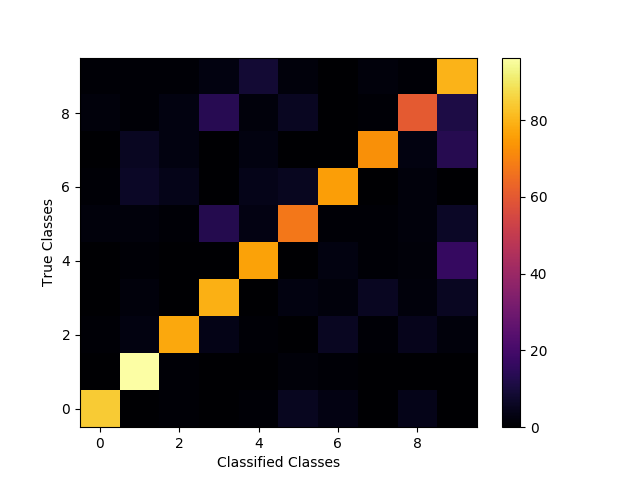
\includegraphics[scale=0.7]{prob1/confusion_mat.png}
   	\caption{Confusion Matrix for Single Pixel Features}
   	\label{fig:cm11}
   \end{figure}

	\begin{figure}[!htb]
		\centering
		\subfloat[Digit 4 Log Likelihood]{{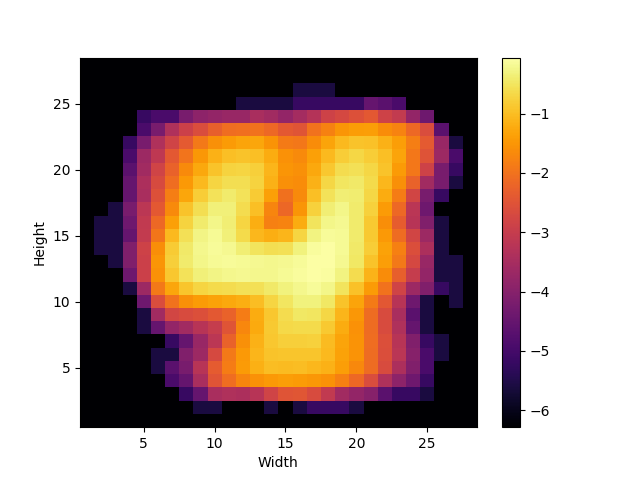
\includegraphics[width=4cm]{prob1/llhd4} }}%
		\qquad
		\subfloat[Digit 9 Log Likelihood]{{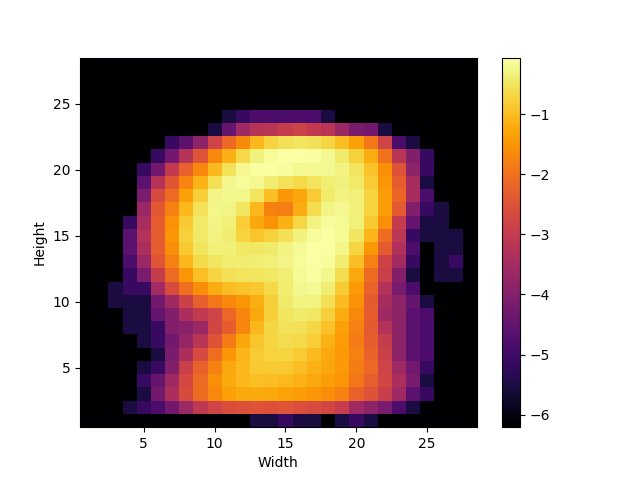
\includegraphics[width=4cm]{prob1/llhd9} }}%
		\qquad
		\subfloat[(4, 9) Log Odd Ratio]{{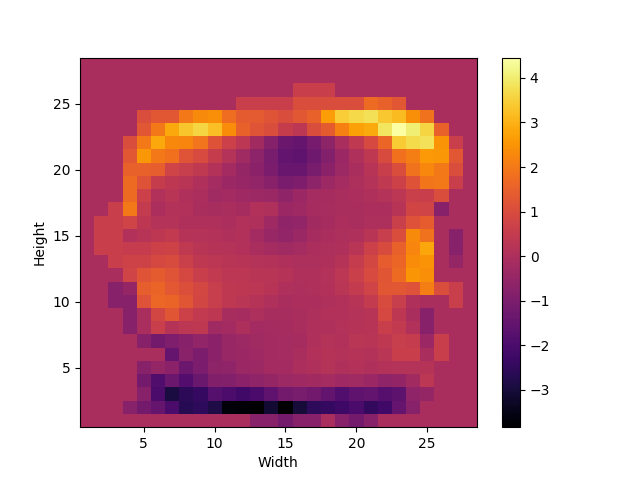
\includegraphics[width=4cm]{prob1/odds_4_9} }}%
		\caption{Log Likelihood and Log Odd Ratio for (4, 9) Misclassification Pair}%
		\label{fig:mdp1}
	\end{figure}

	\begin{figure}[!htb]
		\centering
		\subfloat[Digit 5 Log Likelihood]{{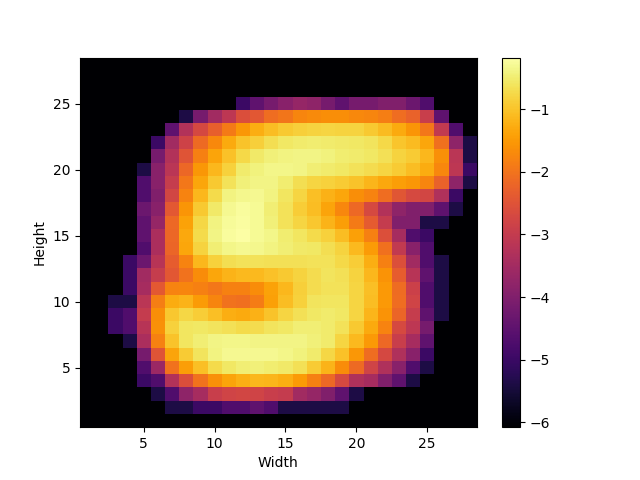
\includegraphics[width=4cm]{prob1/llhd5} }}%
		\qquad
		\subfloat[Digit 3 Log Likelihood]{{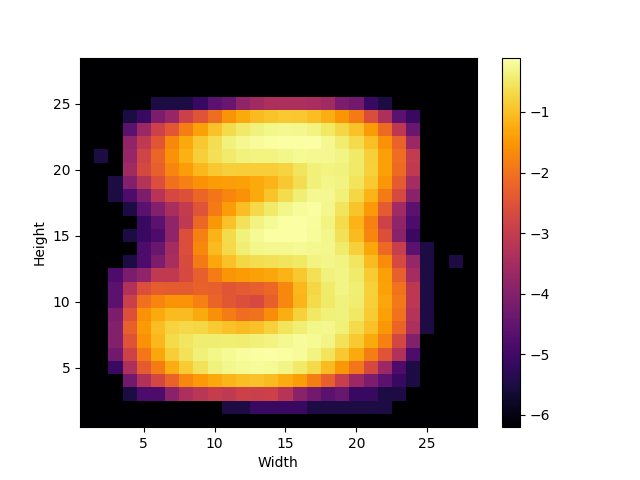
\includegraphics[width=4cm]{prob1/llhd3} }}%
		\qquad
		\subfloat[(5, 3) Log Odd Ratio]{{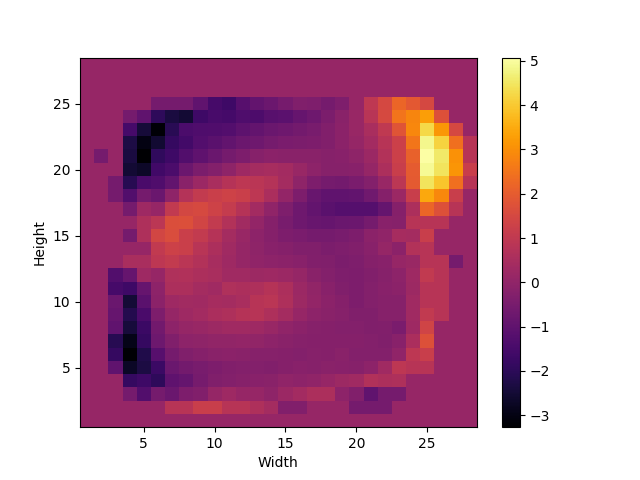
\includegraphics[width=4cm]{prob1/odds_5_3} }}%
		\caption{Log Likelihood and Log Odd Ratio for (5, 3) Misclassification Pair}%
		\label{fig:mdp2}
	\end{figure}

	\begin{figure}[!htb]
		\centering
		\subfloat[Digit 7 Log Likelihood]{{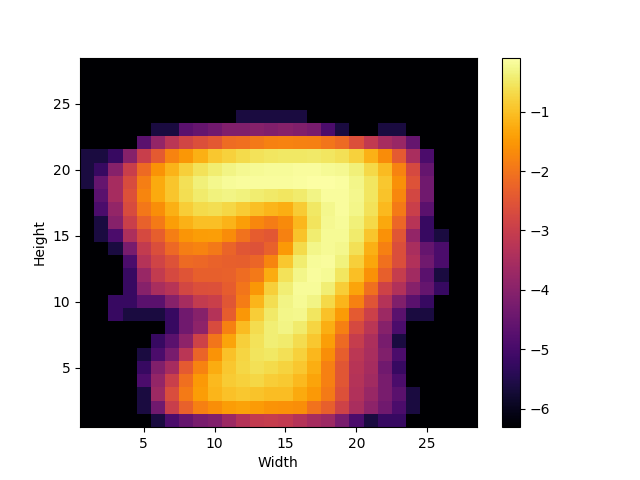
\includegraphics[width=4cm]{prob1/llhd7} }}%
		\qquad
		\subfloat[Digit 9 Log Likelihood]{{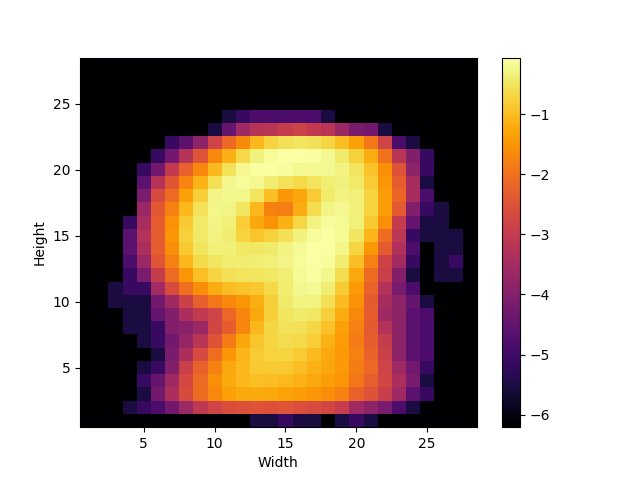
\includegraphics[width=4cm]{prob1/llhd9} }}%
		\qquad
		\subfloat[(7, 9) Log Odd Ratio]{{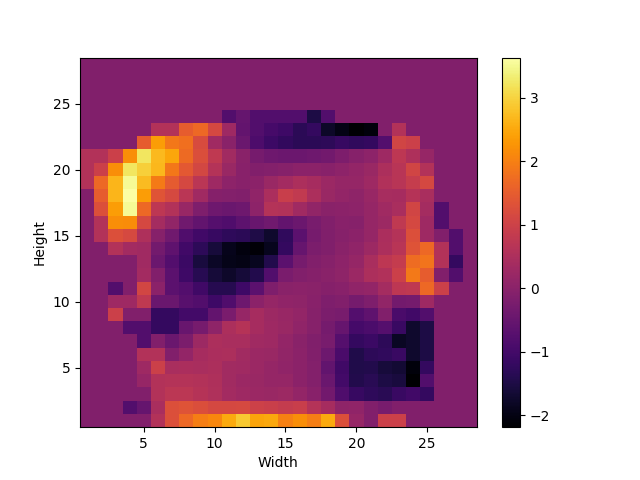
\includegraphics[width=4cm]{prob1/odds_7_9} }}%
		\caption{Log Likelihood and Log Odd Ratio for (7, 9) Misclassification Pair}%
		\label{fig:mdp3}
	\end{figure}

	\begin{figure}[!htb]
		\centering
		\subfloat[Digit 8 Log Likelihood]{{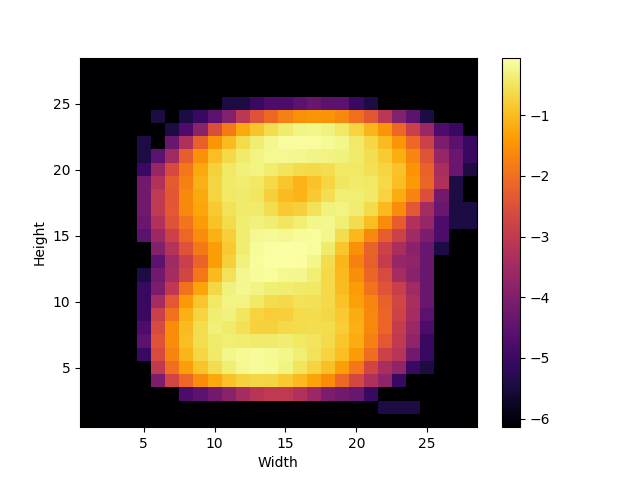
\includegraphics[width=4cm]{prob1/llhd8} }}%
		\qquad
		\subfloat[Digit 3 Log Likelihood]{{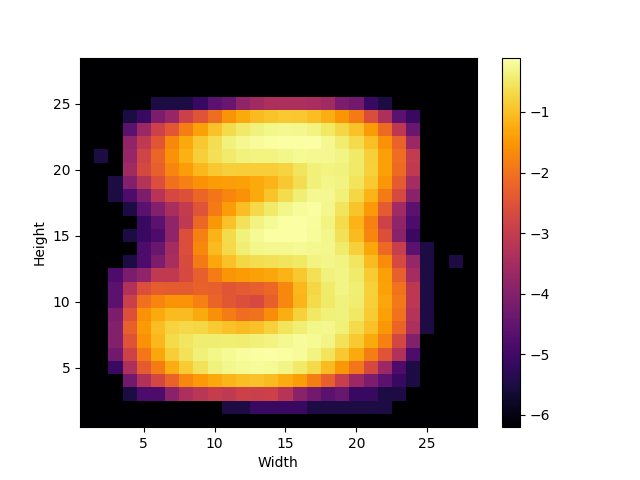
\includegraphics[width=4cm]{prob1/llhd3} }}%
		\qquad
		\subfloat[(8, 3) Log Odd Ratio]{{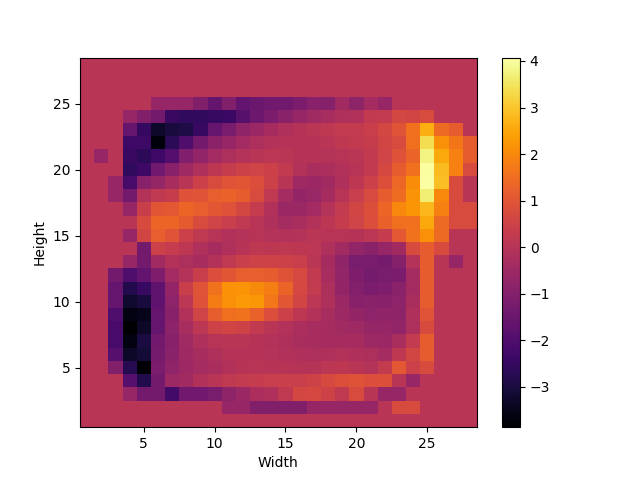
\includegraphics[width=4cm]{prob1/odds_8_3} }}%
		\caption{Log Likelihood and Log Odd Ratio for (8, 3) Misclassification Pair}%
		\label{fig:mdp4}
	\end{figure}
   
   
   \begin{figure}[!htb]
   	\centering
   	\subfloat[Min Posterior Test Data]{{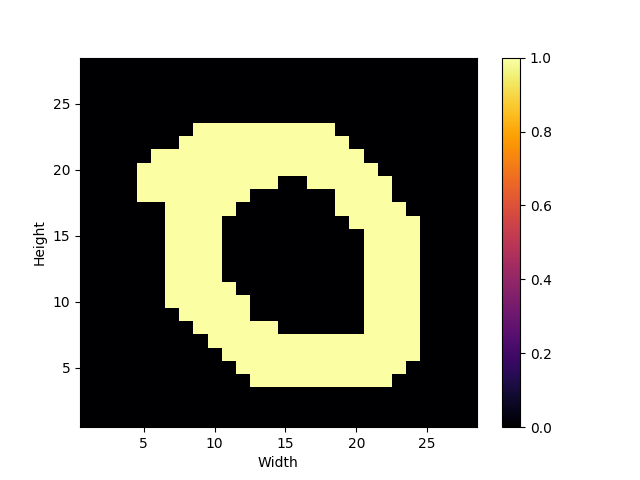
\includegraphics[width=5cm]{prob1/class0_minPosteriorTestData} }}%
   	\qquad
   	\subfloat[Max Posterior Test Data]{{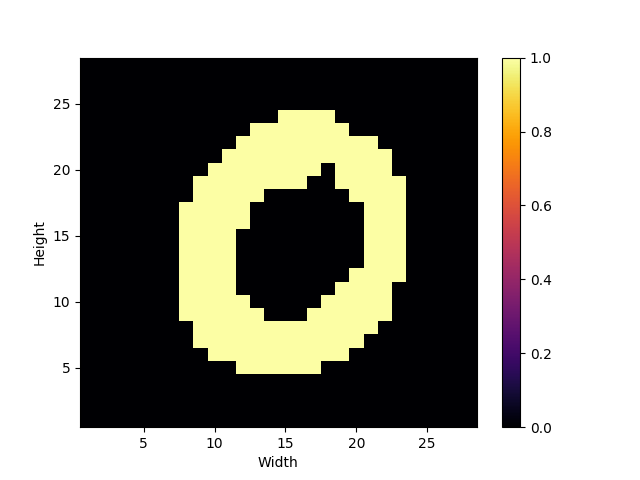
\includegraphics[width=5cm]{prob1/class0_maxPosteriorTestData} }}%
   	\caption{Min and Max Posterior Test Data for 0 Digit}%
   	\label{fig:d0p}
   \end{figure}

\begin{figure}[!htb]
	\centering
	\subfloat[Min Posterior Test Data]{{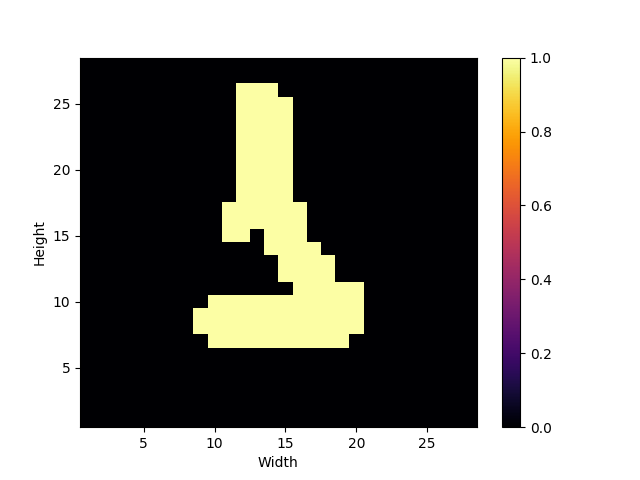
\includegraphics[width=5cm]{prob1/class1_minPosteriorTestData} }}%
	\qquad
	\subfloat[Max Posterior Test Data]{{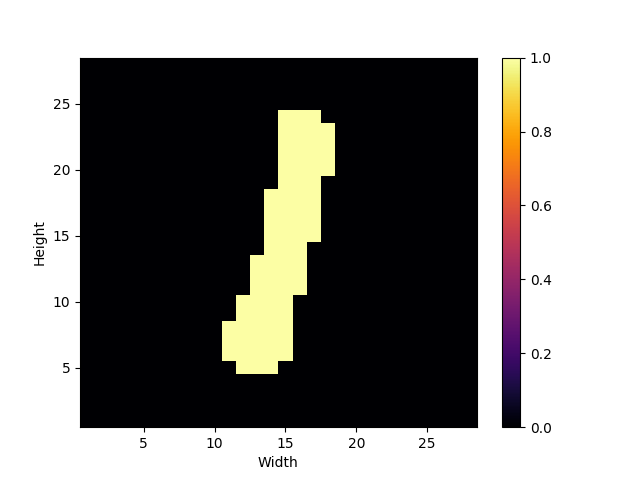
\includegraphics[width=5cm]{prob1/class1_maxPosteriorTestData} }}%
	\caption{Min and Max Posterior Test Data for 1 Digit}%
	\label{fig:d1p}
\end{figure}

\begin{figure}[!htb]
	\centering
	\subfloat[Min Posterior Test Data]{{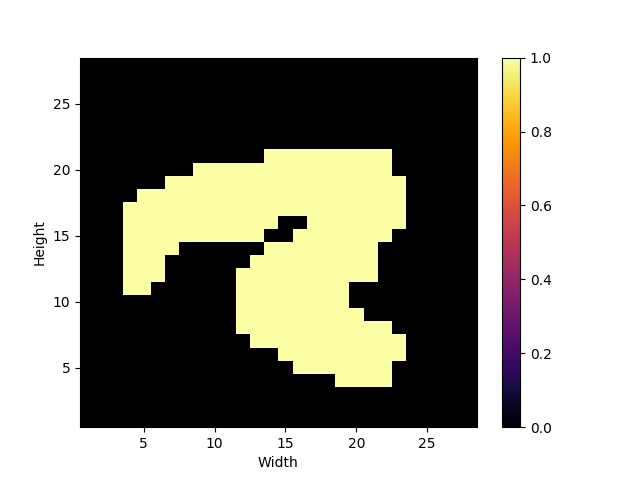
\includegraphics[width=5cm]{prob1/class2_minPosteriorTestData} }}%
	\qquad
	\subfloat[Max Posterior Test Data]{{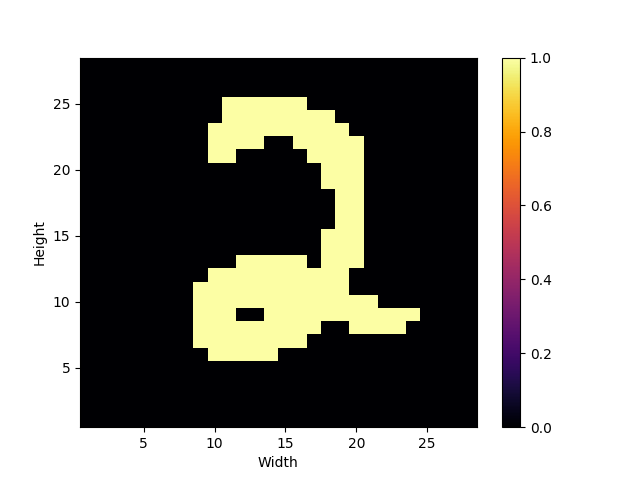
\includegraphics[width=5cm]{prob1/class2_maxPosteriorTestData} }}%
	\caption{Min and Max Posterior Test Data for 2 Digit}%
	\label{fig:d2p}
\end{figure}

\begin{figure}[!htb]
	\centering
	\subfloat[Min Posterior Test Data]{{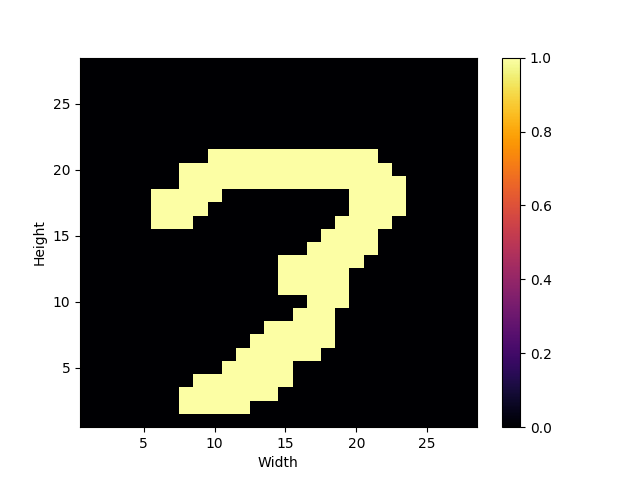
\includegraphics[width=5cm]{prob1/class3_minPosteriorTestData} }}%
	\qquad
	\subfloat[Max Posterior Test Data]{{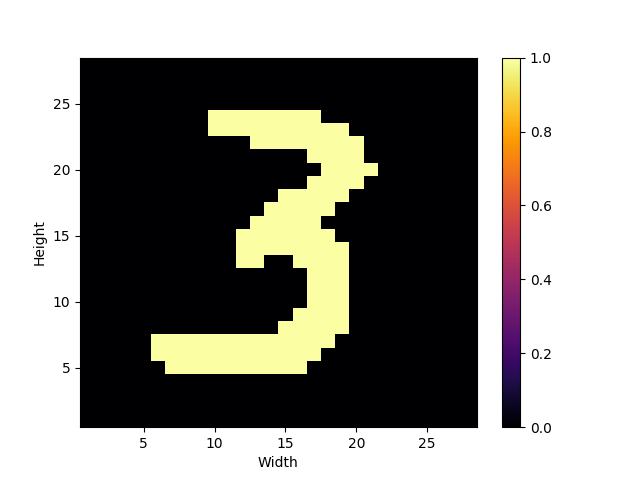
\includegraphics[width=5cm]{prob1/class3_maxPosteriorTestData} }}%
	\caption{Min and Max Posterior Test Data for 3 Digit}%
	\label{fig:d3p}
\end{figure}

\begin{figure}[!htb]
	\centering
	\subfloat[Min Posterior Test Data]{{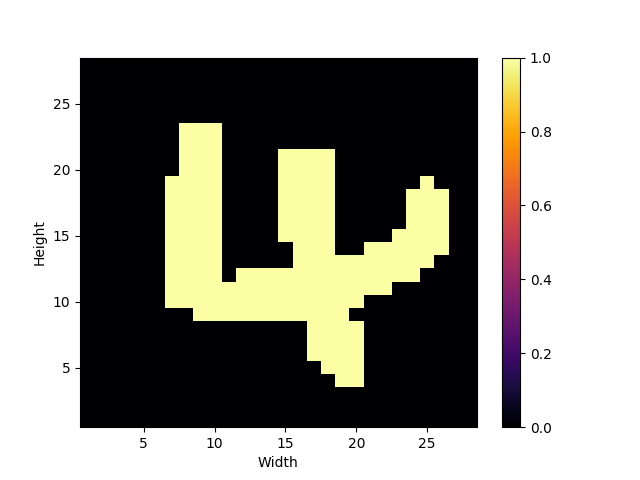
\includegraphics[width=5cm]{prob1/class4_minPosteriorTestData} }}%
	\qquad
	\subfloat[Max Posterior Test Data]{{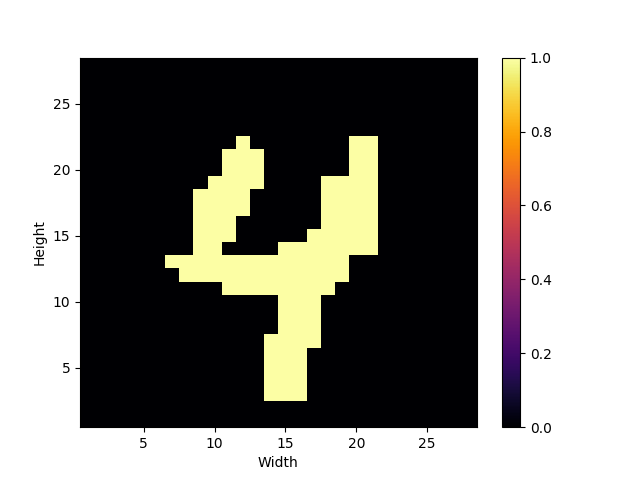
\includegraphics[width=5cm]{prob1/class4_maxPosteriorTestData} }}%
	\caption{Min and Max Posterior Test Data for 4 Digit}%
	\label{fig:d4p}
\end{figure}

\begin{figure}[!htb]
	\centering
	\subfloat[Min Posterior Test Data]{{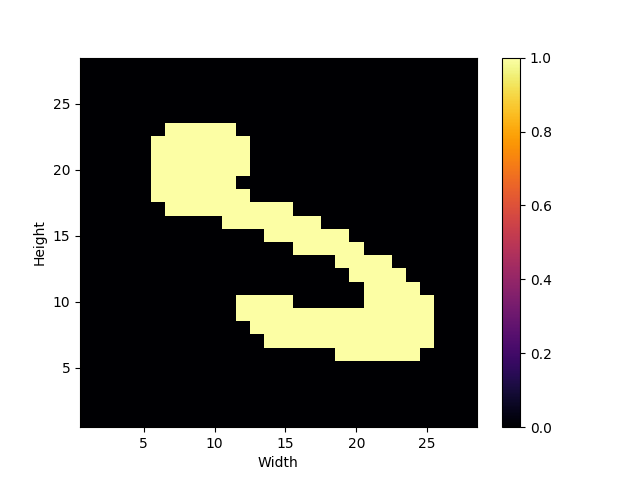
\includegraphics[width=5cm]{prob1/class5_minPosteriorTestData} }}%
	\qquad
	\subfloat[Max Posterior Test Data]{{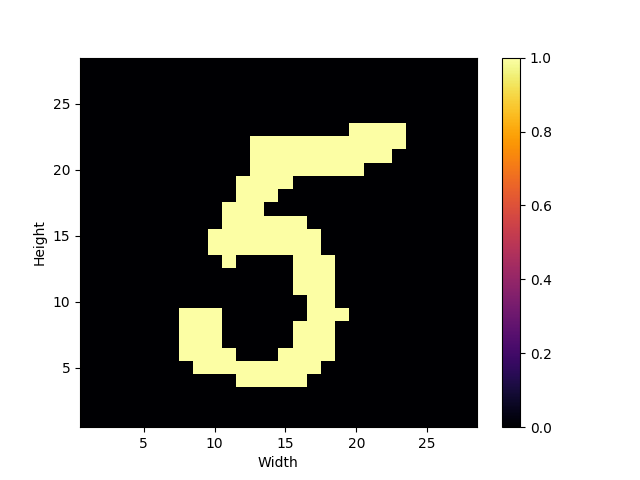
\includegraphics[width=5cm]{prob1/class5_maxPosteriorTestData} }}%
	\caption{Min and Max Posterior Test Data for 5 Digit}%
	\label{fig:d5p}
\end{figure}

\begin{figure}[!htb]
	\centering
	\subfloat[Min Posterior Test Data]{{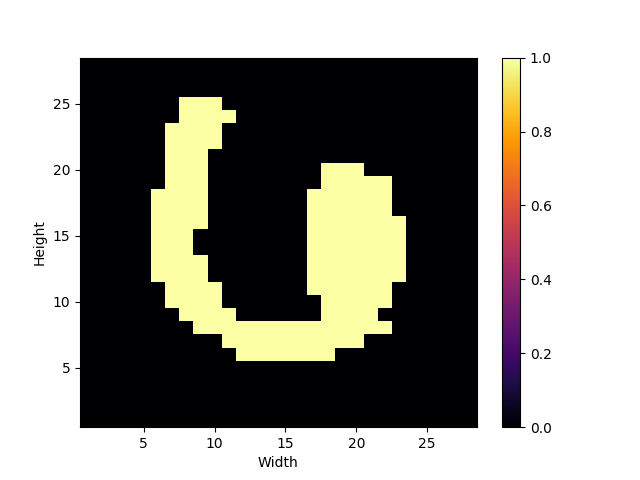
\includegraphics[width=5cm]{prob1/class6_minPosteriorTestData} }}%
	\qquad
	\subfloat[Max Posterior Test Data]{{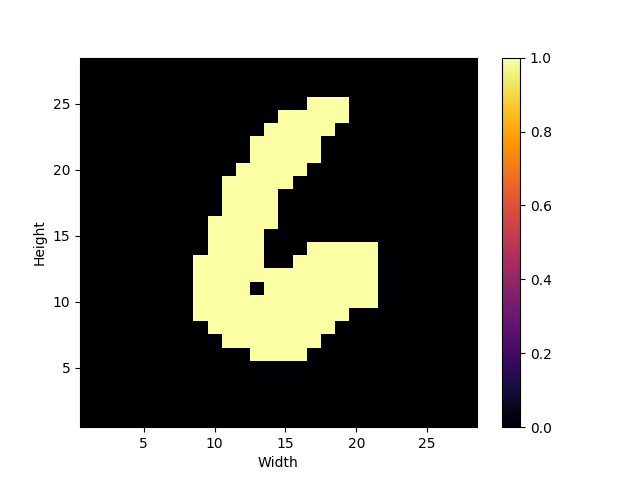
\includegraphics[width=5cm]{prob1/class6_maxPosteriorTestData} }}%
	\caption{Min and Max Posterior Test Data for 6 Digit}%
	\label{fig:d6p}
\end{figure}

\begin{figure}[!htb]
	\centering
	\subfloat[Min Posterior Test Data]{{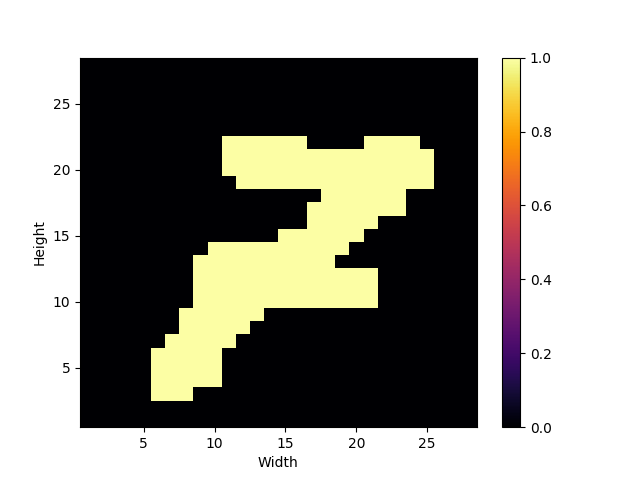
\includegraphics[width=5cm]{prob1/class7_minPosteriorTestData} }}%
	\qquad
	\subfloat[Max Posterior Test Data]{{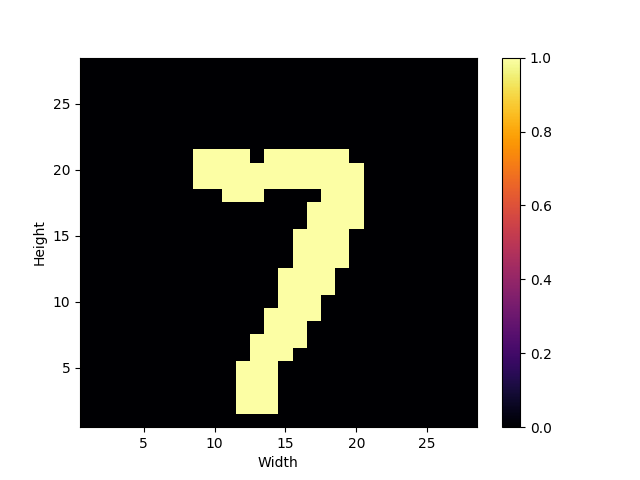
\includegraphics[width=5cm]{prob1/class7_maxPosteriorTestData} }}%
	\caption{Min and Max Posterior Test Data for 7 Digit}%
	\label{fig:d7p}
\end{figure}

\begin{figure}[!htb]
	\centering
	\subfloat[Min Posterior Test Data]{{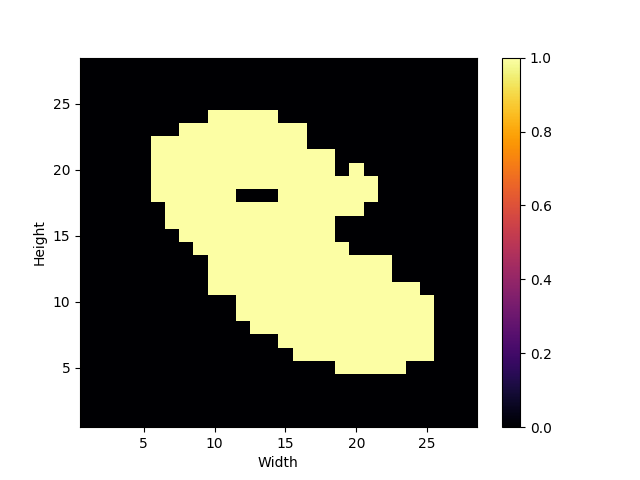
\includegraphics[width=5cm]{prob1/class8_minPosteriorTestData} }}%
	\qquad
	\subfloat[Max Posterior Test Data]{{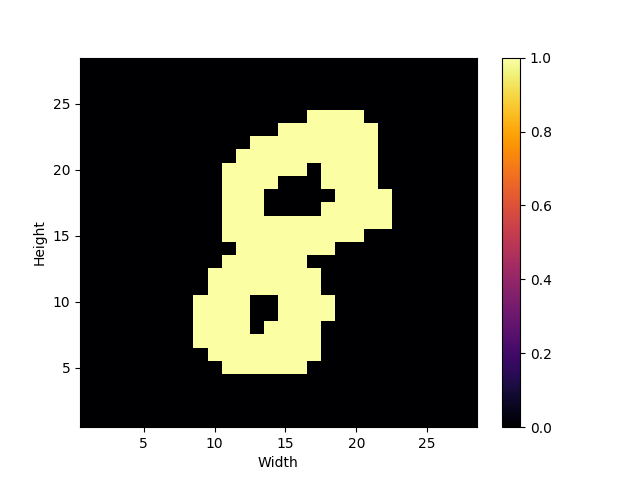
\includegraphics[width=5cm]{prob1/class8_maxPosteriorTestData} }}%
	\caption{Min and Max Posterior Test Data for 8 Digit}%
	\label{fig:d8p}
\end{figure}

\begin{figure}[!htb]
	\centering
	\subfloat[Min Posterior Test Data]{{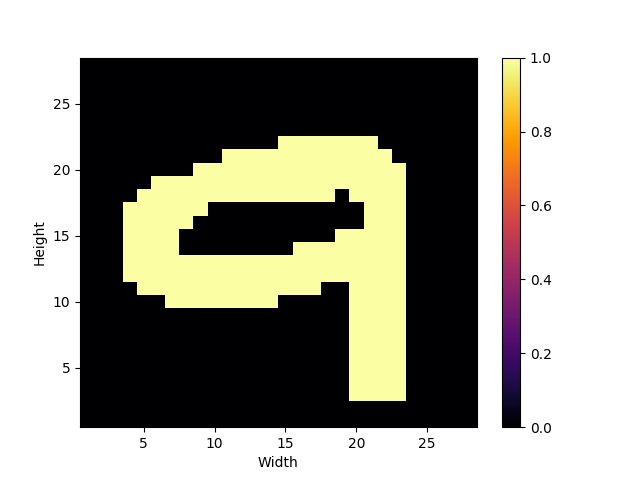
\includegraphics[width=5cm]{prob1/class9_minPosteriorTestData} }}%
	\qquad
	\subfloat[Max Posterior Test Data]{{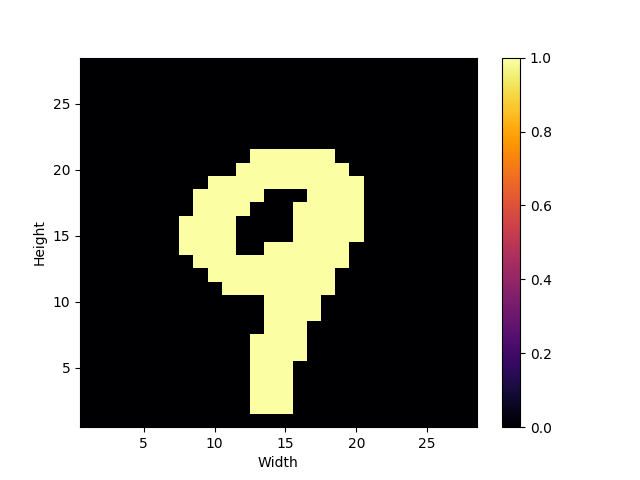
\includegraphics[width=5cm]{prob1/class9_maxPosteriorTestData} }}%
	\caption{Min and Max Posterior Test Data for 9 Digit}%
	\label{fig:d9p}
\end{figure}
   
   
   %%
   %% Subsection about Part 1.2 using features based on a set of disjoint local chunks of image
   %%
  \subsection{Disjoint Block as Features}
  \subsubsection{Problem Formulation} \label{sssec:disform}
  Within this problem, we take the same dataset of square images, each with $n = 28$ rows and columns of pixels with binary values, and create new set of features based on taking disjoint subregions of a given image and representing them as a single value. For simplicity, each image $I \in B_I = \lbrace 0,1 \rbrace^{n \times n}$ and define $V_{rq} = \lbrace 0, 1, \cdots, 2^{rq}-1 \rbrace$. Then let us define the operator $F_{rq}: B_I \rightarrow V_{rq}^{\frac{n}{r} \times \frac{n}{q}}$ as the map that converts an image into a smaller matrix made up of the new, disjoint features. The algorithm representing $F_{rq}$ for computing the new set of features is found in Algorithm \ref{algo:fdisjoint}.
  
  \RestyleAlgo{boxruled}
  \begin{algorithm}[ht]
  	\caption{$F_{rq}$ Definition }
  	\KwData{Image, $I \in B_I$ }
  	\KwData{Number of rows in subblock of image used for a feature, $r$ }
  	\KwData{Number of columns in subblock of image used for a feature, $q$ }
  	\KwResult{Output matrix of new features, $G \in V_{rq}^{\frac{n}{r} \times \frac{n}{q}}$}
  	\;
  	
  	\tcp{Initialize output feature matrix, $G$}
  	$G_{ij} = 0$  $\forall i \in \lbrace 1, 2, \cdots, \frac{n}{r}\rbrace, j \in \lbrace 1, 2, \cdots, \frac{n}{q} \rbrace $
  	\;
  	\;
  	
  	\tcp{Construct the feature values}
  	\For{$i \in \lbrace 1, 2, \cdots, \frac{n}{r}\rbrace$}{
  		\For{$j \in \lbrace 1, 2, \cdots, \frac{n}{q} \rbrace$}{
  			\For{$k \in \lbrace 1, 2, \cdots, r \rbrace$}{
  				\For{$l \in \lbrace 1, 2, \cdots, q \rbrace$}{
  					$t = 1 + (i-1)r + k$ \;
  					$s = 1 + (j-1)q + l$ \;
  					$G_{ij} = G_{ij} + 2^{(l-1) + q (k-1)} I_{ts}$
  				}
  			}
  		}
  	}
  	\;
  	
  	\Return $G$
  	\label{algo:fdisjoint}
  \end{algorithm}
  
  For ease of use, each resulting feature matrix $G$ is vectorized into a column vector such that $V = V_{rq} $ and $d = \frac{n^2}{rq}$ for some chosen pair of $r$ and $q$, given the definitions in Section \ref{sec:one}. Using this formulation, we can again use the generic algorithms based on the formulation in Section \ref{sec:one} to compute the information needed for the classifier.
  
  \subsubsection{Results} \label{sssec:disres}
  For the results generated, we are looking at features with dimension pairs (2,2), (2,4), (4,2), and (4,4). With this set of disjoint block feature dimensions, Table \ref{tab:dis} includes the accuracy and training run-time for each pair, including (1,1) which represents the data collected in Section \ref{ssec:spf}.
  
  \begin{table}[ht]
  	\centering
  	\begin{tabular}{l | l | l | l}
  		\hline
  		Feature Dimension Pair & Training Run-time & Testing Run-time & Accuracy  \\
  		\hline \hline 
  		(1, 1) & 0.155s & 18.08s &77.1\% \\
  		(2, 2) & 0.194s & 4.082s &84.3\% \\
  		(2, 4) & 1.609s & 2.156s &82.7\% \\
  		(4, 2) & 1.734s & 2.036s &84.7\% \\
  		(4, 4) & 183.6s & 0.975s &75.3\% \\
  		\hline
  	\end{tabular}
  \caption{Results information for Disjoint Block Features} \label{tab:dis}
  \end{table}
  
  In terms of trends, especially when looking at the features based on individual pixels from Section \ref{ssec:spf}, there are some notable ones. First, we can see that using the disjoint block features, in general, improve performance relative to the individual pixel features. We can also see, however, that making the Disjoint Blocks enclose too many pixels can actually hurt performance, likely because too large of blocks result in too much loss of information and make it hard to make meaningful classifications from that resulting feature dataset. 
  
  If one looks at run-time for training, we can see the block size of the features increases exponentially as the number of pixels per block are increased. This makes sense because, based on the discussion from Section \ref{ssec:ldv}, we can see the run-time complexity for the disjoint block features will be $O\left(\frac{n^2}{rq} 2^{rq} p N\right)$. If we hold other terms constant, we can see that the run-time complexity grows by $\frac{2^{rq}}{rq}$ as the product of the disjoint block dimensions, $rq$, grows. 
  
  For large product values for $rq$, one would expect the exponential numerator to greatly dominate, in turn making large disjoint block features take much longer to train. This analysis validates why the (4,4) feature is much more time consuming to train than the (1,1) feature, while the (2,2) feature is not much slower to train relative to the (1,1) feature.
  
  As for the testing run-time, we know from Section \ref{ssec:ldv} that the complexity will be $O\left(p\frac{n^2}{rq}\right)$. This means that as $rq$ increases, we should expect the run-time to decrease dramatically due to the $(rq)^{-1}$ factor. Looking at the results from Table \ref{tab:dis}, we can see this reduction occurs as the disjoint blocks span a wider area of pixels, validating the theoretical analysis.
  
  %%
  %% Subsection about Part 1.2 using features based on a set of disjoint local chunks of image
  %%
   \subsection{Overlapping Block as Features}
   \subsubsection{Problem Formulation}
   Similarly to the Disjoint Block features, we take the same dataset of square images, each with $n = 28$ rows and columns of pixels with binary values, and create new set of features based on taking overlapping subregions of a given image and representing them as a single value. For simplicity, each image $I \in B_I = \lbrace 0,1 \rbrace^{n \times n}$ and define $V_{rq} = \lbrace 0, 1, \cdots, 2^{rq}-1 \rbrace$. Then let us define the operator $H_{rq}: B_I \rightarrow V_{rq}^{(n-r+1) \times (n-q+1)}$ as the map that converts an image into a smaller matrix made up of the new, overlapping features. The algorithm representing $H_{rq}$ for computing the new set of features is found in Algorithm \ref{algo:fover}.
   
   \RestyleAlgo{boxruled}
   \begin{algorithm}[H]
   	\caption{$H_{rq}$ Definition }
   	\KwData{Image, $I \in B_I$ }
   	\KwData{Number of rows in subblock of image used for a feature, $r$ }
   	\KwData{Number of columns in subblock of image used for a feature, $q$ }
   	\KwResult{Output matrix of new features, $G \in V_{rq}^{(n-r+1) \times (n-q+1)}$}
   	\;
   	
   	\tcp{Initialize output feature matrix, $G$}
   	$G_{ij} = 0$  $\forall i \in \lbrace 1, 2, \cdots, (n-r+1)\rbrace, j \in \lbrace 1, 2, \cdots, (n-q+1) \rbrace $
   	\;
   	\;
   	
   	\tcp{Construct the feature values}
   	\For{$i \in \lbrace 1, 2, \cdots, (n-r+1)\rbrace$}{
   		\For{$j \in \lbrace 1, 2, \cdots, (n-q+1) \rbrace$}{
   			\For{$k \in \lbrace 1, 2, \cdots, r \rbrace$}{
   				\For{$l \in \lbrace 1, 2, \cdots, q \rbrace$}{
   					$t = (i+k)$ \;
   					$s = (j+l)$ \;
   					$G_{ij} = G_{ij} + 2^{(l-1) + q (k-1)} I_{ts}$
   				}
   			}
   		}
   	}
   	\;
   	
   	\Return $G$
   	\label{algo:fover}
   \end{algorithm}
   
   As before, each resulting feature matrix $G$ is vectorized into a column vector such that $V = V_{rq} $ and $d = (n-r+1)(n-q+1)$ for some chosen pair of $r$ and $q$, given the definitions in Section \ref{sec:one}. Using this formulation, we can again use the generic algorithms based on the formulation in Section \ref{sec:one} to compute the information needed for the classifier.
   
   \subsubsection{Results}
   For the results generated, we are looking at features with dimension pairs (2,2), (2,4), (4,2), (4,4), (2,3), (3, 2), (3,3). With this set of overlapping block feature dimensions, Table \ref{tab:ovr} includes the accuracy and training run-time for each pair, including (1,1) which represents the data collected in Section \ref{ssec:spf}.
   
   \begin{table}[ht]
   	\centering
   	\begin{tabular}{l | l | l | l}
   		\hline
   		Feature Dimension Pair & Training Run-time & Testing Run-time & Accuracy  \\
   		\hline \hline 
   		(1, 1) & 0.155s & 18.08s &77.1\% \\
   		(2, 2) & 0.739s & 14.43s & 85.4\% \\
   		(2, 4) & 11.13s & 16.75s & 85.4\% \\
   		(4, 2) & 11.75s & 13.59s & 85.9\% \\
   		(4, 4) & 2,516s & 13.26s & 80.3\% \\
   		(2, 3) & 2.869s & 13.33s & 86.0\% \\
   		(3, 2) & 2.610s & 13.42s & 86.9\% \\
   		(3, 3) & 20.52s & 13.02s & 83.7\% \\
   		\hline
   	\end{tabular}
   	\caption{Results information for Overlapping Block Features} \label{tab:ovr}
   \end{table}
   
   When looking at the features based on individual pixels from Section \ref{ssec:spf} and the disjoint feature results in Section \ref{sssec:disres}, there are some notable trends. First, we can see that the Overlapping Block features achieve more robust accuracies, all block sizes achieving 80\%+ performance. This trend makes sense since the Overlapping Block features ensure we don't miss much information, even with larger block sizes, due to the overlapping behavior. We also note that there is a sweet spot in terms of block dimensions that achieves performance of just under 87\%. What I find interesting is how, based on reviewing the (2,4), (4,2), (2,3), (3,2) results, it appears that features that represent blocks with more rows perform better than blocks with more columns, implying vertical information is less important than the horizontal information.
   
   If one looks at run-time for training, we can see the block size of the features increases exponentially as the number of pixels per block are increased. This makes sense because, based on the discussion from Section \ref{ssec:ldv}, we can see the run-time complexity for the overlapping block features will be $O(n^2 2^{rq} p N)$. If we hold other terms constant, we can see that the run-time complexity grows proportionally to $2^{rq}$ as the product of the overlapping block dimensions, $rq$, grows. Note that this growth is larger than the growth seen in the disjoint block as a function of $rq$. This model explains why the (4,4) feature is much more time consuming to train than the (1,1) feature, while the (2,2) feature is not much slower to train relative to the (1,1) feature. The larger time complexity growth seen by the overlapping block as a function of $rq$ also explains why the run-time is much slower for each block feature dimension when contrasting it to the corresponding disjoint features.
   
   As for the testing run-time, we know from Section \ref{ssec:ldv} that the complexity will be $O\left(p n^2\right)$. This means that as the dimensions of the overlapping block features change, we should not expect the run-time to change much. Looking at the results from Table \ref{tab:dis}, we can see that for most of the overlapping features, the testing run-time is similar to each other, validating the theoretical analysis.
   
   \section{Problem 1 Extra Credit | Face Classification}
   The problem being tackled here is taking dataset of labeled thresholded images, based on some edge detection computer vision algorithm, and learning to classify images as either a Face (1) or a Non-face (0). 
   
   \subsubsection{Problem Formulation}
   This problem was formulated identically to the formulation found in Section \ref{sssec:disform} for the disjoint block features. All work done there carries over into here. One thing to note is that $\Omega = \lbrace 0, 1\rbrace$ where, as stated before, the face label is 1 and the non-face label is 0. Additionally, a disjoint block size of (2,2) was used to reduce the resolution of the input matrix of data while also keeping a sufficient amount of information. The Laplace Smoothing constant was set to $\alpha = 0.1$.
   
   \subsubsection{Results}
   After training and testing, it was found that using (2,2) disjoint features produced a classification accuracy on the testing dataset of 98\%. The confusion matrix for this test dataset can be seen in Figure \ref{fig:cm1face}, making it obvious this classifier performed well against the training dataset.
   
   \begin{figure}[!htb]
   	\centering
   	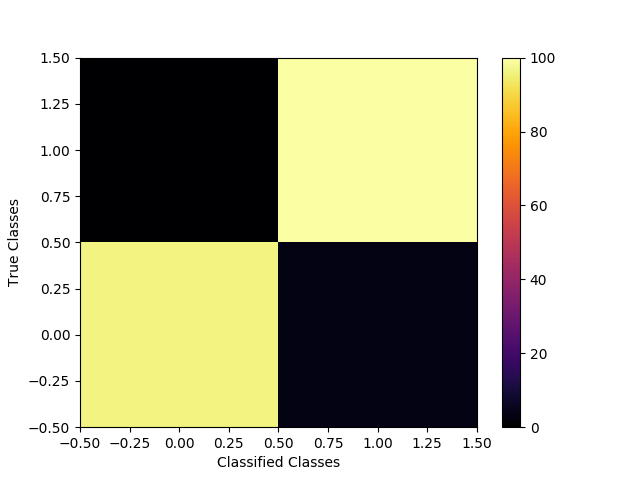
\includegraphics[scale=0.7]{prob1_face/confusion_mat.png}
   	\caption{Confusion Matrix for Face Dataset using (2,2) Disjoint Block Features}
   	\label{fig:cm1face}
   \end{figure}
   
   \newpage
   \section{Part 2 | Audio Classification}
   \subsection{Classification of Hebrew 'Yes' and 'No'}
   Within this problem, the goal is to create a classifier that can distinguish between recordings saying the words 'Yes' and 'No' in Hebrew. The sounds are all represented as thresholded spectrograms, meaning that again the data will be read into memory with binary feature values. 
   
   \subsubsection{Problem Formulation}
   Within this problem, we take a dataset of thresholded spectrograms matrices, each with $n_r = 25$ rows and $n_c = 10$ columns of binary values, and vectorize this matrix for use in our framework defined in Section \ref{sec:one}. Doing this gives us $V = \lbrace 0, 1 \rbrace $ and $d = n_c n_r$, given the definitions in Section \ref{sec:one}. Note that we also define $\Omega = \lbrace 0, 1\rbrace$, where $0$ is a label for 'No' and $1$ is a label for 'Yes'. Using this formulation, it is straight forward to use our generic algorithms to build and test a classifier for this problem.
   
   \subsubsection{Results}
   After training and testing the classifier based on the spectrogram data, it was found that the classifier correctly classified 96\% of the testing data. This is after messing around with the Laplace Smoothing constant, $\alpha$, and finding that the performance really didn't change as a function of the constant, so I chose $\alpha = 0.1$. The confusion matrix for the results can be found in Figure \ref{fig:cm21}. Recall again that the $0$ label is for 'No' and the $1$ label is for 'Yes'. It is visually obvious from the confusion matrix that there is minimal errors in the classification. I suspect that the Hebrew 'Yes' and 'No' words have sufficiently different pronunciations to make the classifier this strong.
   
   \begin{figure}[!htb]
   	\centering
   	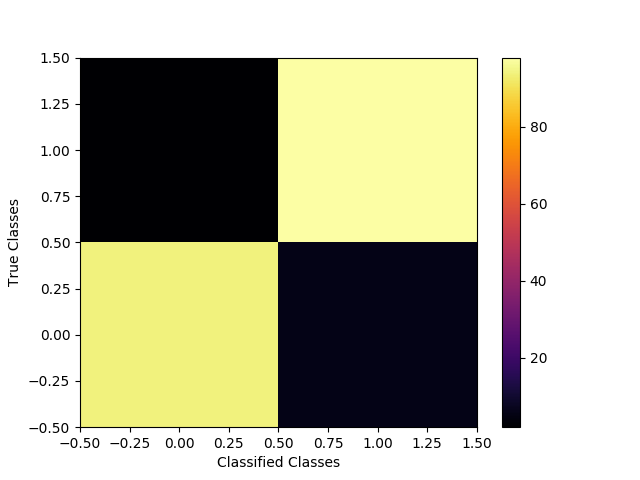
\includegraphics[scale=0.7]{prob21/confusion_mat.png}
   	\caption{Confusion Matrix for Hebrew 'Yes' vs 'No' Classification}
   	\label{fig:cm21}
   \end{figure}
   
   
   
   \subsection{Classification of Spoken Digits}
   Within this problem, the goal is to create a classifier that can distinguish between different digits, particularly digits 1 through 5, based on recordings from a set of different speakers. The data given to us is a labeled set of thresholded Mel-frequency Cepstrum Coefficients (MFCCs). The goal is to create a classifier that can achieve greater than 80\% overall classification accuracy. 
   
   \subsubsection{Problem Formulation}
   For practical purposes, the MFCCs we are given are essentially matrices with binary values for each element of the matrices. If we take each matrix, with $n_r = 30$ rows and $n_c = 13$ columns of binary values, we can vectorize this matrix for use in our framework defined in Section \ref{sec:one}. Doing this gives us $V = \lbrace 0, 1 \rbrace $ and $d = n_c n_r$, given the definitions in Section \ref{sec:one}. Note that we also define $\Omega = \lbrace 1, 2, 3, 4, 5 \rbrace$, where each of the labels correspond to the spoken digit we are classifying. Using this formulation, it is straight forward to use our generic algorithms to build and test a classifier for this problem.
   
   \subsubsection{Results}
   After training and testing the classifier based on the spectrogram data, it was found that the classifier correctly classified 85\% of the testing data. The confusion matrix for the results can be found in Figure \ref{fig:cm22}. Based on the confusion matrix, it appears the digits that were toughest to correctly classify were 4 and 5. Particularly, there was a large misclassification error where the classifier interpreted some of the data labeled 4 as a 2. Additionally, noticeably large misclassification errors occurred with 5 where the classifier interpreted some of the data labeled 5 as 1 or 3.
   
   \begin{figure}[!htb]
   	\centering
   	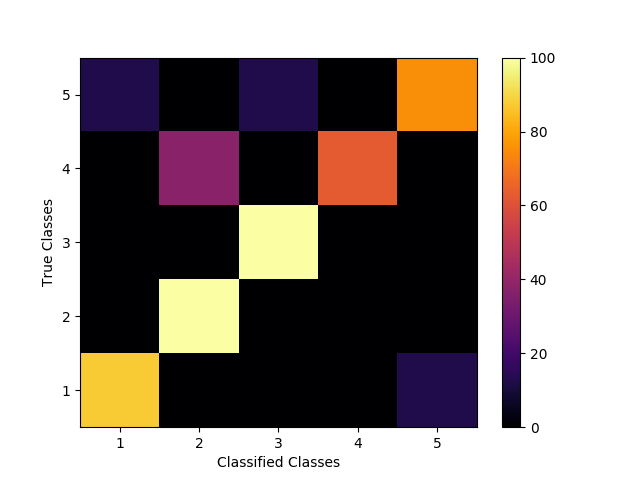
\includegraphics[scale=0.7]{prob22/confusion_mat.png}
   	\caption{Confusion Matrix for Spoken Digit Classification}
   	\label{fig:cm22}
   \end{figure}

\newpage
\section{Contributions}
\begin{itemize}
\item Christian Howard
	\begin{itemize}
	\item Did everything since worked on this MP alone
	\end{itemize}
\end{itemize}   
   
   
\newpage
   \section{List of Potential Extra Credit}
   \begin{itemize}
   \item Face Classification for Part 1 of the assignment
\end{itemize}      
   
   \newpage
\begin{appendices}

   \section{Open Source Software Used}
   Some system python libraries, as well as the \textbf{numpy} package, were used to help develop the codes used in this MP.

\end{appendices}   
   
   
   
\end{document}